\documentclass{beamer}

%\usepackage{beamerthemesidebar, fancybox}
\usepackage{beamerthemesplit,fancybox}
%\usepackage[pdftex]{color,graphicx}
\usepackage{graphicx,pgfarrows,pgfnodes}
%\usepackage{pgfarrows,pgfnodes}
\usepackage{verbatim} % for block comments, so I can comment out entire slides easily

%\usepackage{pgfpages}
%\pgfpagesuselayout{resize}[a4paper,border shrink=5mm,landscape]

\usepackage{mjclectureslides}


\definecolor{Dblue}{rgb}{.255,.41,.884}

\title[Preliminaries: set notation, counting]{Introduction to Probability \\ Introduction to set notation, \\
combinatorial analysis (counting)}
%\author[Prof. Michael Carlisle]{Prof. Michael Carlisle}
%\institute{Baruch College, CUNY}
%\date{Spring 2018}
\date{} 

\begin{document}

\frame{\titlepage}

\frame{ \frametitle{Introduction}

The point of this course is to understand the notion of \textbf{probability} and to develop the ability to reason, calculate, and formulate problems in a probabilistic way.

\vspace{5mm}

To start, here are some key words that should guide your thought processes throughout the semester. In all situations, we consider ``experiments'' where there are multiple possible results. 

}


\frame{ \frametitle{Key words to keep in mind}

\begin{itemize}
\item \textbf{set, event}: the basic mathematical tool for collecting and differentiating all the ``possible things'' we are considering.
\vspace{3mm}
\item \textbf{count}: the simplest way to say ``how many different things'' we are considering, when the number of things to consider is finite. 
\vspace{3mm}
\item \textbf{measure}: an abstracted notion of ``size'' when ``counting'' can't be done, i.e. with infinite-size sets.
\vspace{3mm}
\item \textbf{ratio}: fraction. percentage. a \emph{part of a whole} of ``how many different things'' we are considering. 
\vspace{3mm}
\item \textbf{condition}: ``evidence'' can narrow down the possible things available to a problem.
\end{itemize}

}



\frame{ \frametitle{Set / Element}

We start with the basic definitions of set notation.

\vspace{5mm}

\begin{defn} A \textbf{set} is a collection of distinct objects, called the set's \textbf{elements}. 

\vspace{5mm}

The elements:
\begin{itemize}
\item do not necessarily have an inherent order or relationship to each other (although they usually will); 
\item duplicates are not allowed; 
\item they are merely \emph{different things in the same bag}. 
\end{itemize}
\end{defn}

}


\frame{ \frametitle{Set / Element Notation}

``The set $A$ contains three elements: 

\begin{center}
`cat', `tree', and the number 6.''
\end{center}

This is denoted 
\[ A = \{ \text{tree}, \text{cat}, 6 \} \]

\vspace{3mm}

with curly brackets indicating the set.

\vspace{5mm}

This is an \emph{explicit} definition of a particular set. It has 3 elements.

\vspace{5mm}

``6 is an element of $A$'' is denoted $6 \in A$.\\

\vspace{5mm}

``'dog' is not an element of $A$'' is denoted dog $\not \in A$. 

}



\frame{ \frametitle{Set / Element Notation}

``The set $B$ consists of the even numbers \emph{strictly} between 0 and 25'' 
(i.e. \emph{exclusive}) is an \emph{implicit} definition of the set denoted 

\vspace{3mm}

\[ B = \{ 2, 4, 6, ..., 22, 24\}. \]

\vspace{5mm}

The \emph{ellipsis} ``...'' means: 

\begin{center}
``you understand the pattern given by the context''.
\end{center}

}


\frame{ \frametitle{Set / Element Notation}

Another way to write

\vspace{3mm}

\[ B = \{ 2, 4, 6, ..., 22, 24\} \]

\vspace{3mm}

is 

\vspace{3mm}

\[ B = \{ x \in \mathbb{Z} \, | \, 0 < x < 25, \, x \text{ even}\}, \]

\vspace{3mm}

where the vertical bar $|$ means ``such that''. 

\vspace{3mm}

(Sometimes a colon : is used instead of the bar $|$.)

}



\frame{ \frametitle{Popular Number Sets}

$\mathbb{N} = \{ 1, 2, 3, ... \}$ is the set of \textbf{natural numbers} \\
or \textbf{counting numbers} (and sometimes contains 0). 

\vspace{10mm}

$\mathbb{Z} = \{ ..., -3, -2, -1, 0, 1, 2, 3, ... \}$ is the set of \textbf{integers} \\
(written with a Z for the German word Zahlen (``numbers'')). 

\vspace{10mm}

 $\mathbb{Q} = \{ \frac{m}{n} \, | \, m, n \in \mathbb{Z}, \, n \neq 0 \}$ is the set of \textbf{rational numbers} \\
 (i.e. fractions, ratios; the Q stands for ``quotient''). 

}


\frame{ \frametitle{Real Number Sets}

$\mathbb{R}$ is the set of \textbf{real numbers}, containing all rational and irrational numbers. This is the set of numbers along the continuous number line, containing all infinite-length decimal expansions. 

\vspace{4mm}

\begin{figure}[!ht]
  \centering
    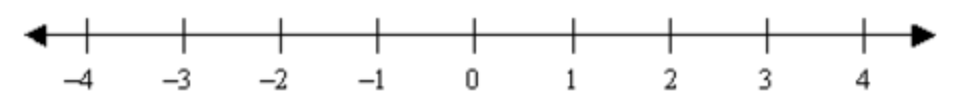
\includegraphics[width=4in]{numberline.png}
\end{figure}

\vspace{4mm}

An \textbf{open interval} of real numbers is denoted 

\[ (a, b) = \{ x \in \mathbb{R} : a < x < b \}. \]

\vspace{3mm} 

A \textbf{closed interval} of real numbers is denoted 

\[ [a, b] = \{ x \in \mathbb{R} : a \leq x \leq b \}. \]

}




\frame{ \frametitle{Cardinality}

The \textbf{cardinality} of a set is the number of (distinct) elements of the set. 
The cardinality of the set $A$ is denoted $|A|$ or $\#A$. 

\vspace{5mm}

\textbf{Finite} sets have an obvious cardinality: count the elements. 

\vspace{5mm}

Examples: $|\{ 4, 6, 2, 9 \}| = 4$, $|\{ 7, 8, ..., 100 \}| = 94$. 

\vspace{5mm}
%\onslide<2->


\textbf{Infinite} sets are more complicated to deal with. 

}


\frame{ \frametitle{Infinite Cardinality and Sums/Integrals}

We will not trouble ourselves with the details here, except to mention that the ``smallest'' level is called \textbf{countable infinity}.

\vspace{5mm}

We can sum a countable number of items, and they may or may not converge.

\vspace{5mm}

Consider the geometric series: if $|x| < 1$, the sum of the numbers 
\[ x^0 = 1, \,\, x^1 = x, \,\, x^2, \,\, x^3, \,\, ... \] 
is 
\[ \sum_{n=0}^{\infty} x^n = 1 + x + x^2 + x^3 + ... = \frac{1}{1-x}. \]
The cardinality of the real numbers $\R$ is called \textbf{uncountable}, and we cannot sum this many values; we need integrals for that.

}


\frame{ \frametitle{Venn diagrams}

A \textbf{Venn diagram} (named after John Venn (1834-1923)) is a simple graphic displaying the overlap of different sets.

\vspace{5mm}

We use Venn diagrams to help understand problems in counting, probability, logic, and other fields. 

\vspace{5mm}

We'll sketch some diagrams for two sets $A$ and $B$, sharing the same universal set $U$ (the box surrounding them).

}


\frame{ \frametitle{Empty Set}

The \textbf{empty set} is the set with no elements (think: an empty bag). 

\vspace{5mm}

It is denoted 

\[ \emptyset \] 

and defined with curly brackets by 

\[ \emptyset = \{\}. \]

The cardinality of the empty set is 

\[ |\emptyset| = 0. \]

}


\frame{ \frametitle{Union}


Some basic operations we can use on sets are: 

\vspace{5mm}

The \textbf{union} of the sets $A$ and $B$ is the set of all elements of $A$ and $B$ combined. It is denoted $A \cup B$, and defined by 

\[ A \cup B = \{ x : \, x \in A \text{ or } x \in B \text{ (or both)}\}. \]

\begin{figure}[!ht]
  \centering
    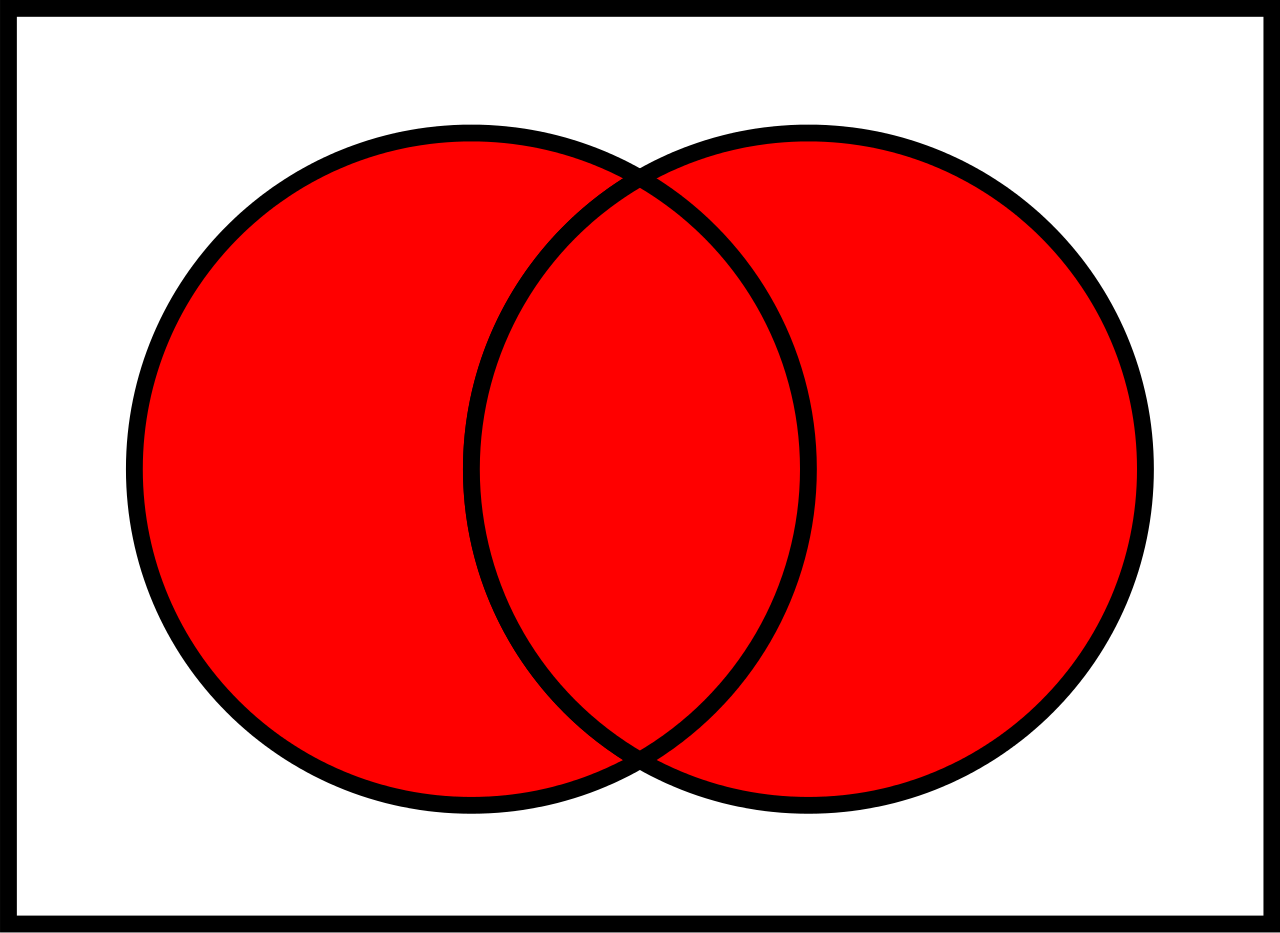
\includegraphics[width=2in]{union.png}
\end{figure}


}


\frame{ \frametitle{Intersection}

The \textbf{intersection} of the sets $A$ and $B$ is the shared elements of $A$ and $B$. It is denoted $A \cap B$ or $AB$, and defined by 

\[ A \cap B = \{ x : \, x \in A \text{ and } x \in B \}. \]

\begin{figure}[!ht]
  \centering
    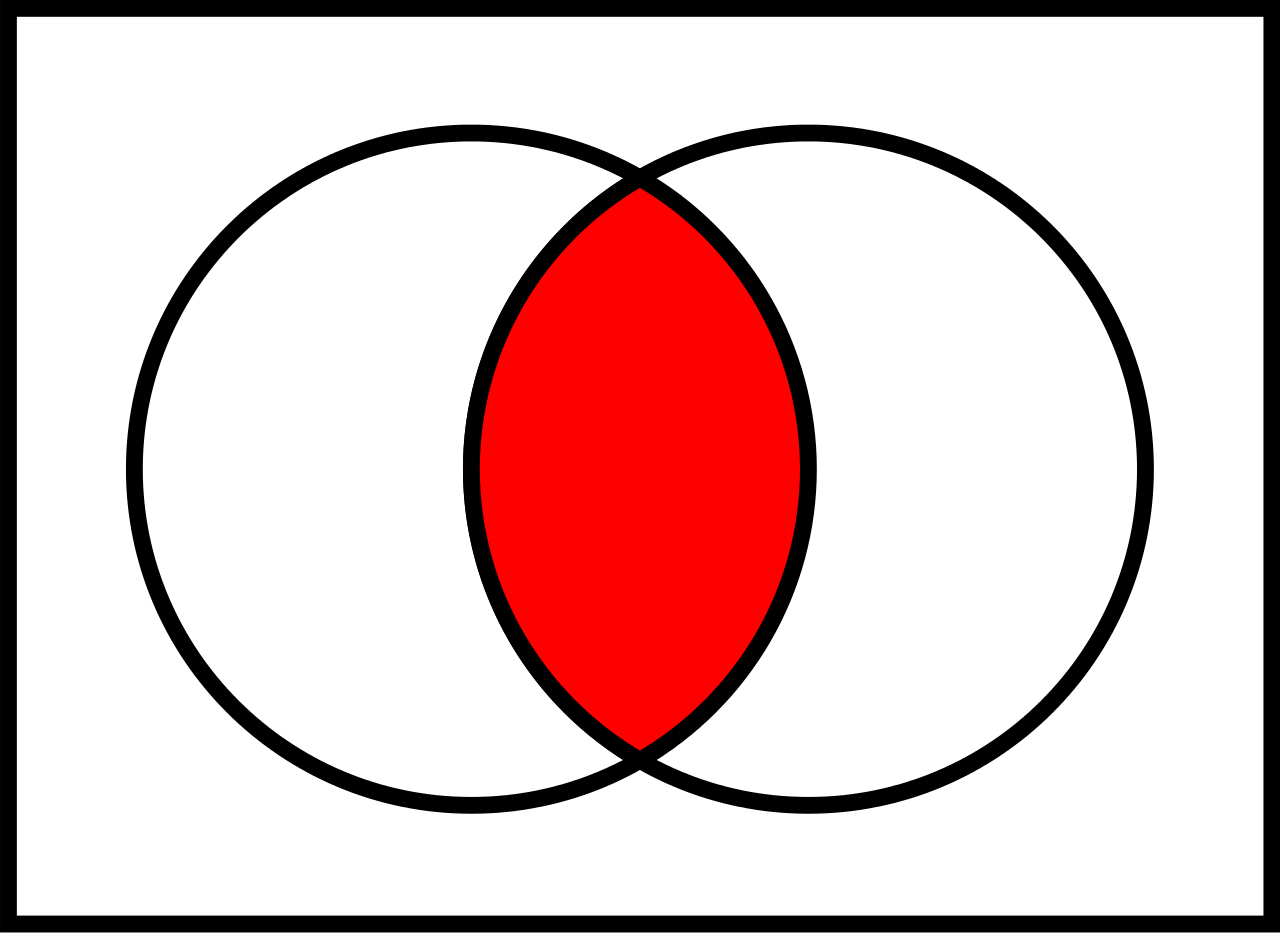
\includegraphics[width=2in]{intersection.png}
\end{figure}

If $A$ and $B$ have no common elements, we say $A$ and $B$ are \textbf{disjoint} sets and denote this fact by  $A \cap B = \emptyset$.

}



\frame{ \frametitle{Set Difference}

The \textbf{set difference} $B \setminus A$ (sometimes denoted $B - A$) is the elements of $B$ with the shared elements of $A$ removed. It is denoted 
\[ B \setminus A = \{ x : \, x \in B \text{ and } x \not \in A \}. \]

\begin{figure}[!ht]
  \centering
    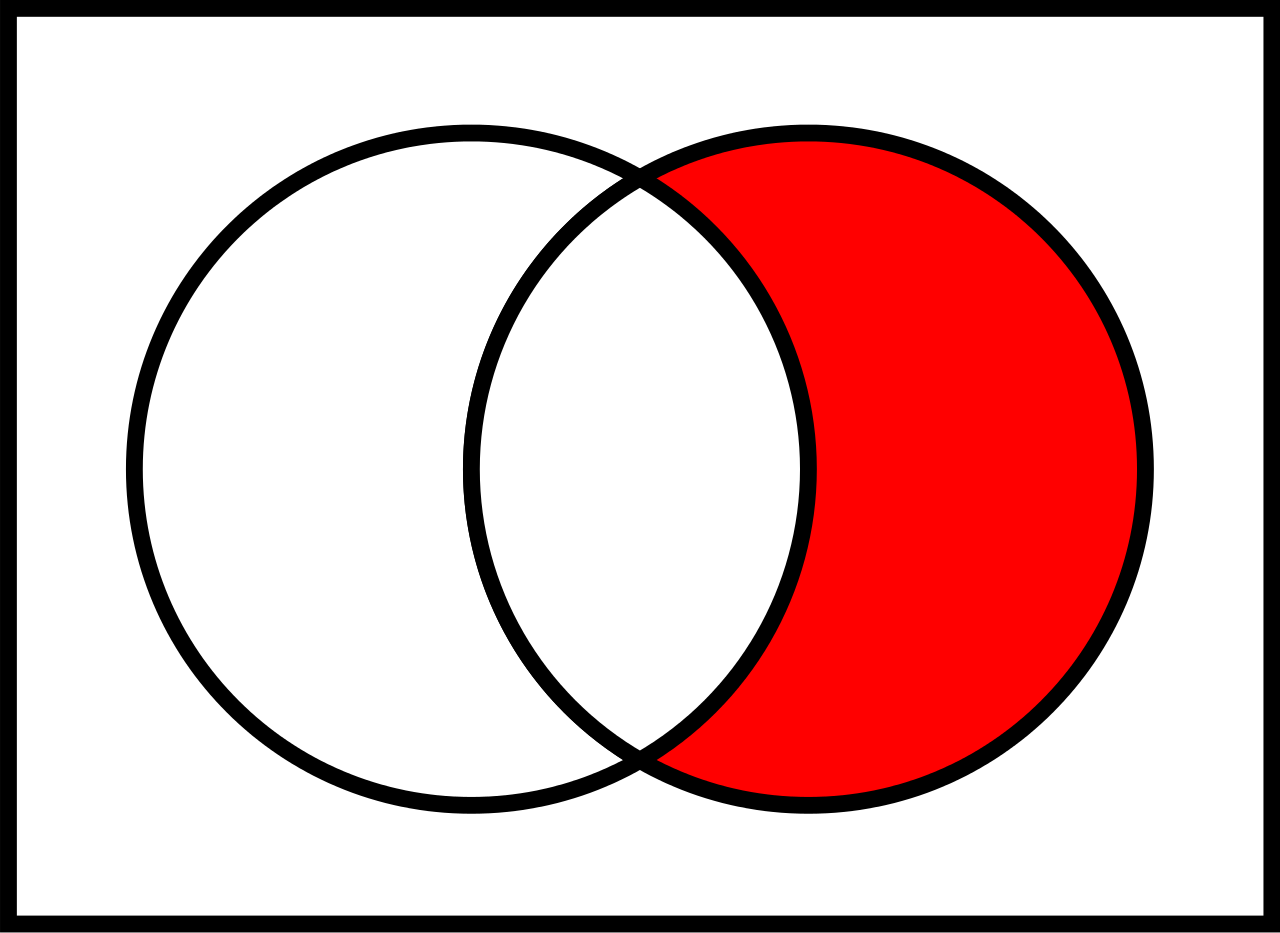
\includegraphics[width=2in]{BminusA.png}
\end{figure}

}


\frame{ \frametitle{Set Difference}

\[ A = \{ 1, 2, 5, 6, 7\}, \,\,\, B = \{ 2, 5, 8, 9, 13\} \]

\[ \implies A \setminus B = \{ 1, 6, 7\} \text{ but } B \setminus A = \{8, 9, 13\}. \]

\begin{figure}[!ht]
  \centering
    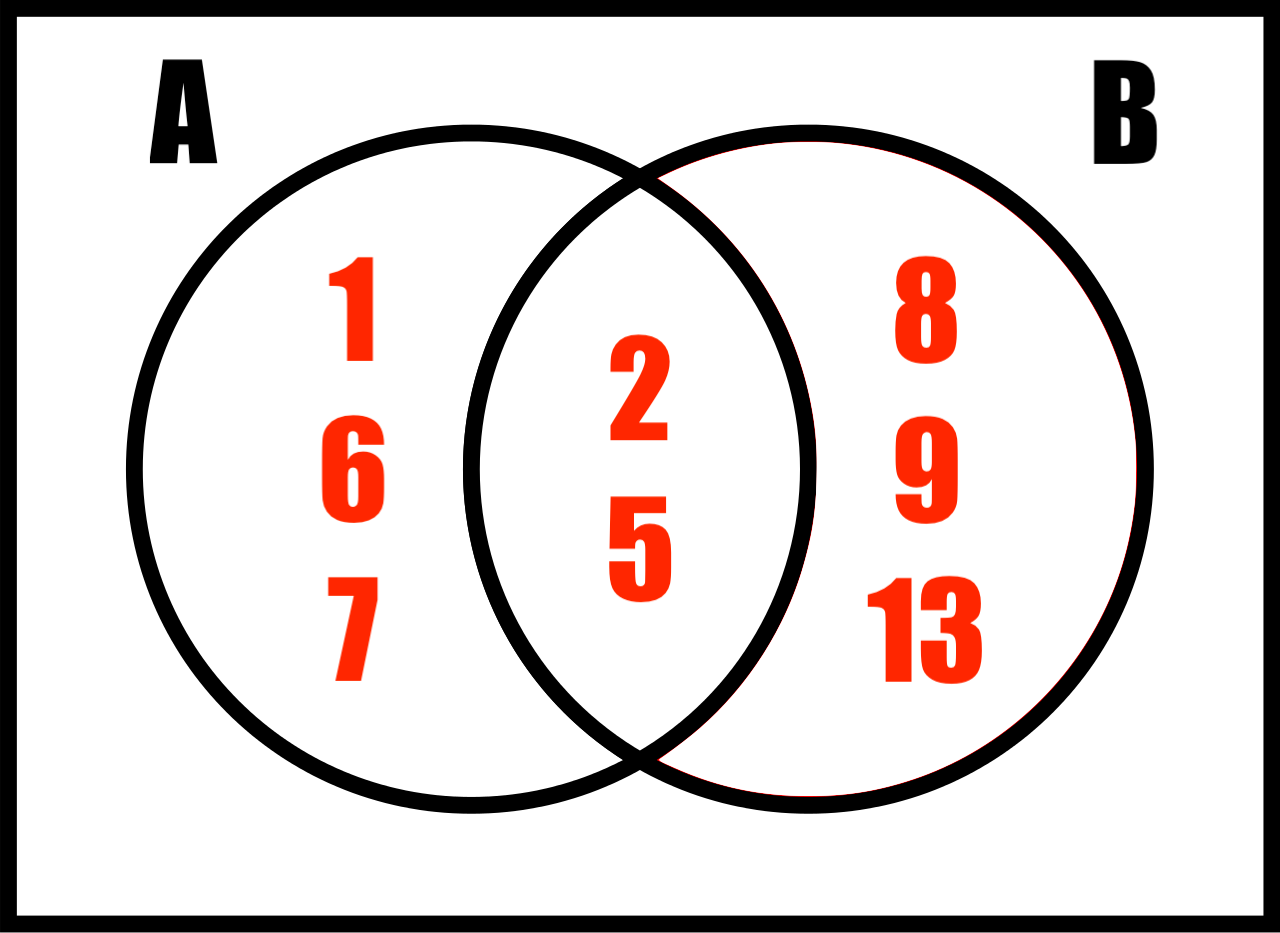
\includegraphics[width=2in]{BminusAexample.png}
\end{figure}

\begin{center}
Thus, $A \setminus B \neq B \setminus A$ (an important general result). 
\end{center}

}


\frame{ \frametitle{Subset}

The set $A$ is called a \textbf{subset} of $B$, denoted $A \subseteq B$, if all of $A$'s elements are in $B$. 
\[ A \subseteq B \iff (x \in A \implies x \in B). \]
\begin{figure}[!ht]
  \centering
    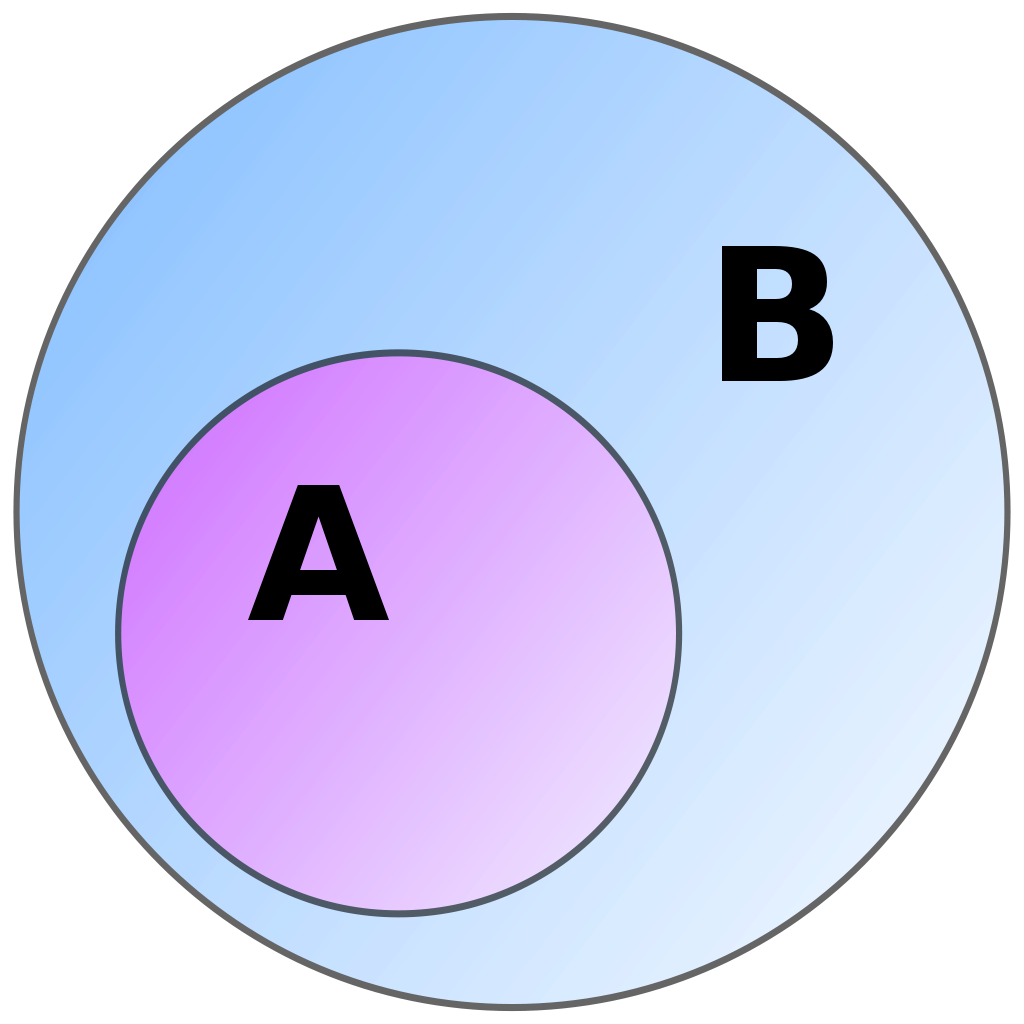
\includegraphics[width=2in]{AsubsetB.png}
\end{figure}

Two sets $A$ and $B$ are \textbf{equal} (written $A = B$) if $A \subseteq B$ and $B \subseteq A$.

}


\frame{ \frametitle{Universal Set, Complement}

In certain collections of problems, we may define a \textbf{universal set} as a common ``top-level set'' under which all the sets described in the problem are subsets of. 

\begin{figure}[!ht]
  \centering
    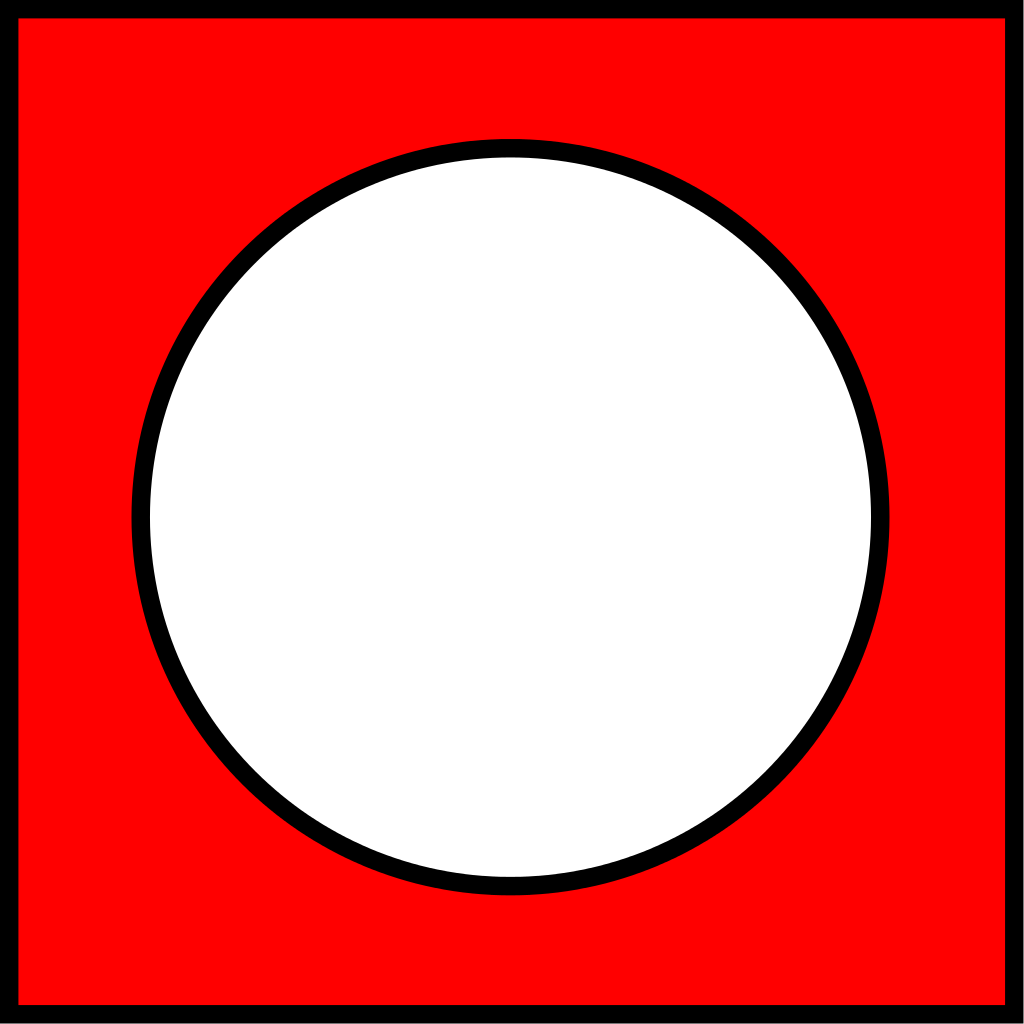
\includegraphics[width=2in]{Acomplement.png}
\end{figure}

}


\frame{ \frametitle{Universal Set, Complement}

The \textbf{complement} of a set $A$, relative to the universal set $U$, is denoted $A^C = U \setminus A$. (Some texts use $A'$ or $\overline{A}$.)

\begin{figure}[!ht]
  \centering
    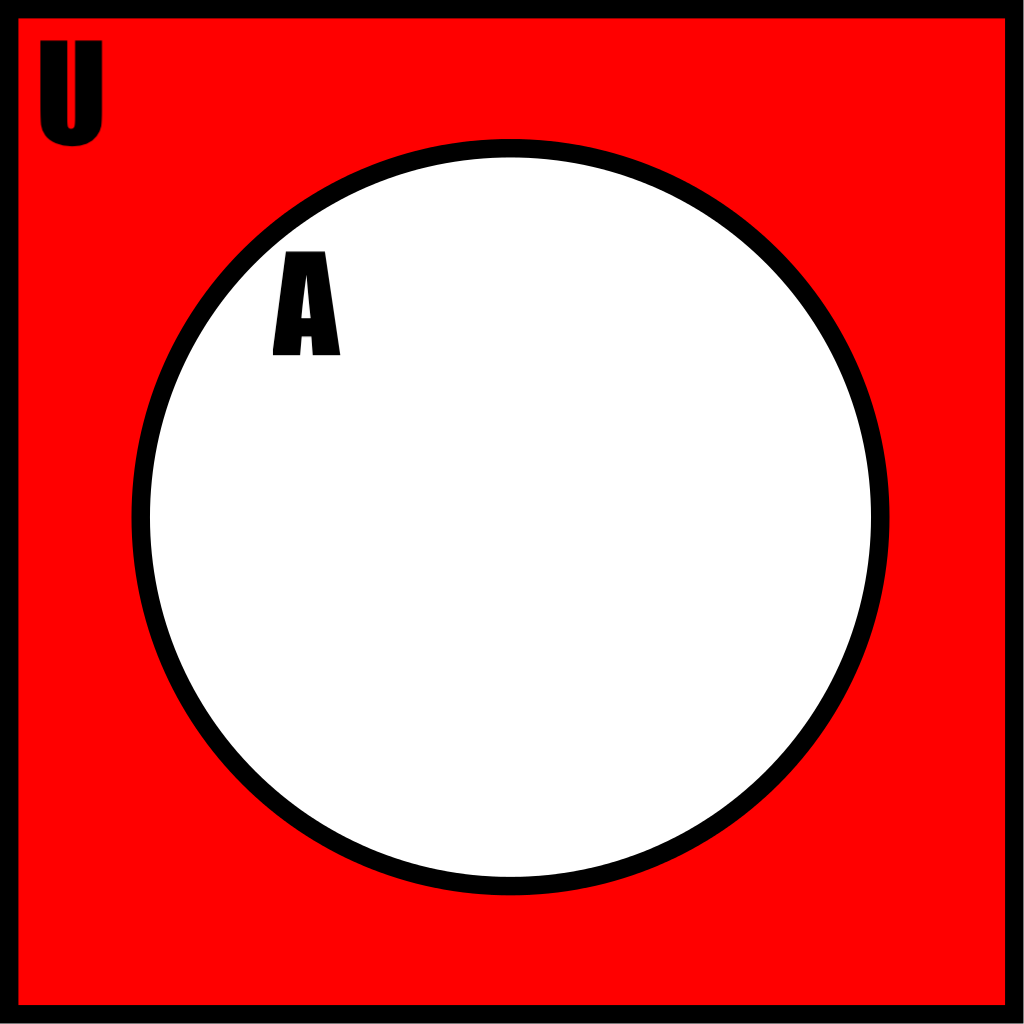
\includegraphics[width=2in]{Acomplement2.png}
\end{figure}

Using this, we can define the set difference as $A \setminus B = A \cap B^C$. 

}



\frame{ \frametitle{Example: Deck of Cards}

\begin{ex}
Say we have a number of questions about a deck of cards. 

\vspace{5mm}

The universal set for these questions could be written as $U$, \\
the set of cards in a standard playing deck: 
\[ U = \{ A\heartsuit, 2\heartsuit, ..., J\heartsuit, Q\heartsuit, K\heartsuit, ... Q\spadesuit, K\spadesuit \}, \]
where $|U| = 52$.

\vspace{5mm}

Let $E = \{ \clubsuit \text{ cards} \}$. Then $E^C = \{ \diamondsuit, \heartsuit, \spadesuit \text{ cards} \}$, and $|E^C| = 39$. 
\end{ex}

\vspace{5mm}

% cardinality of power set, write down a bunch of sets, play with unions, intersections, set differences, symmetric difference, power sets, ... 


}


\frame{ \frametitle{Example: intervals in $\R$}

Considering $\R$ as the universal set, and let 
\vspace{5mm}
\[ A = (1,\infty) = \{ x \in \R: x > 1\}. \]
\vspace{5mm}
Then 
\vspace{5mm}
\[ A^C = \R \setminus A = (-\infty, 1] = \{ x \in \R: x \leq 1\}. \]

}


\frame{ \frametitle{Unions, Intersections, Complements}

Union and intersection are \emph{commutative} operations: 
\vspace{5mm}
\[ A \cup B = B \cup A, \,\, A \cap B = B \cap A. \]

\vspace{5mm}

We've already seen that set difference is \emph{not} commutative: 

\vspace{5mm}

\[ A \setminus B \neq B \setminus A. \]

}


\frame{ \frametitle{Unions, Intersections, Complements}

Union and intersection are also \emph{associative}: 
\vspace{5mm}
\[ (A \cup B) \cup C = A \cup (B \cup C), \,\, (A \cap B) \cap C = A \cap (B \cap C). \]

\vspace{5mm}

Regardless of universal set, it should be clear that the complement of a complement is the original set: 

\vspace{5mm}

\[ (A^C)^C = A. \]

}


\frame{ \frametitle{Distributivity, DeMorgan's Laws}

The \textbf{distributive property} describes how unions and intersections work together: 

\[ (A \cap B) \cup C = (A \cup C) \cap (B \cup C) \]
\[ (A \cup B) \cap C = (A \cap C) \cup (B \cap C) \]

\vspace{5mm} 

%\onslide<2->

\textbf{DeMorgan's Laws} describe the complements of unions and intersections. Complementation flips a union or intersection: 

\[ (A \cap B)^C = A^C \cup B^C \]
\[ (A \cup B)^C = A^C \cap B^C \]

These rules make more obvious sense with \textbf{Venn diagrams} \\
(which we have seen a few of already).

}


\frame{ \frametitle{Probability Terms in Set Theory}

Probability theory has its own set terminology. 

\vspace{5mm} 

A universal set of possible results of a random experiment (often denoted $S$ or $\Omega$) is usually called a \textbf{sample space}. 

\vspace{5mm} 

The elements $\omega \in \Omega$ are called \textbf{outcomes}. 

\vspace{5mm} 

Subsets $E \subseteq \Omega$ are called \textbf{events}. 

}




\frame{ \frametitle{Set (Cartesian) Product, Sequences}

The \textbf{Cartesian product} of two sets $A$ and $B$, denoted $A \times B$, is the set whose elements are \textbf{ordered pairs} $(a,b)$, where $a \in A$ and $b \in B$. 

\vspace{5mm}
%\onslide<2->

Likewise, the Cartesian product of $n$ sets $A_1, A_2, ..., A_n$, denoted $A_1 \times A_2 \times \cdots \times A_n$ or $\prod_{i=1}^n A_i$, is the set whose elements are \textbf{ordered $n$-tuples} $(a_1, a_2, ..., a_n)$, where $a_i \in A_i$ for $i=1,2,...,n$. 

\vspace{5mm}

If $A_1 = A_2 = \cdots = A_n = A$, we can write the product as $A^n$. 

\vspace{5mm}
%\onslide<3->

Note that \emph{order matters} in a Cartesian product of sets: in general, 
\[ A \times B = B \times A \iff A = B. \]


}


\frame{ \frametitle{Cardinality of a Cartesian Product: Multiplication Principle}

The cardinality of a Cartesian product is easy to calculate.

\vspace{5mm}

If $|A| = m$ and $|B| = k$, then it makes sense that the number of items in the product is the product of the individual sets, i.e. 

\vspace{3mm}

\[ |A \times B| = |A| \times |B| = mk. \]

\vspace{5mm}

This property is called the \textbf{Multiplication Principle} of counting.

}


\frame{ \frametitle{Cardinality of a Cartesian Product: Multiplication Principle}

\begin{ex}
There are 6 beverages and 5 entrees to choose from. Disregarding taste, how many ways are there to pair a beverage and an entree? 

\vspace{5mm}

Let $B$ = the set of beverages and $E$ = the set of entrees. Then $|B| = 6$ and $|E| = 5$, and so the total number of possible pairings is 

\vspace{3mm}

\[ |B \times E| = |B| \cdot |E| = 5(6) = 30. \]

\end{ex}
}



\frame{ \frametitle{(Fundamental) Multiplication Principle of Counting}

In general, if 
\[ A_1 \times A_2 \times \cdots \times A_n = \prod_{i=1}^n A_i \]
is the Cartesian product of $n$ sets $A_1, A_2, ..., A_n$, and $|A_i| = m_i$ for $i=1,2,...,n$, then the cardinality of $\prod_{i=1}^n A_i$ is 
\[ \bigg| \prod_{i=1}^n A_i \bigg| = \prod_{i=1}^n |A_i| = \prod_{i=1}^n m_i = m_1 m_2 \cdots m_n. \]

\vspace{5mm}
%\onslide<2->

If $A_1 = A_2 = \cdots = A_n = A$, we can write the product as $A^n$, and if $|A| = m$, then the cardinality of $A^n$ is 
\[ |A^n| = |A|^n = m^n. \]


}



\frame{ \frametitle{Tree Diagrams}

Sometimes the number of possible cases you are to consider in a problem is not a Cartesian product; certain cases do not apply. 

\vspace{5mm}

A simple, graphical way to count in these kinds of problems is with a \textbf{decision tree}. 

}


\frame{ \frametitle{Tree Diagrams}

\textbf{The method:} 
\begin{enumerate}
\item First, start with a ``root'' vertex. 
\item Pick an ordering that makes sense for how to list the possible cases in the problem at hand. 

(It makes sense to use an \emph{unrestricted} set of choices first, and \emph{restricted} choices later.) 

\item For the first set of cases, draw edges (called ``branches'') out from the root counting the number of possible cases, and make vertices for those choices. 

Then, for each later set of choices (restricted ones), draw branches out from each original vertex. 
\item When you've written out all choices, count the number of ``leaves'' (vertices on the ends). 

That's the number of cases for your problem.
\end{enumerate} 

}


\frame{ \frametitle{Multiplication Principle, Decision Trees, Combined Events}

Decision trees can get complex very quickly. 

\vspace{5mm}

We can use the multiplication principle to write out the number of possible cases of a \textbf{combined event}, such as selecting multiple items out of separate groups. 

\vspace{5mm}

As we find more complex ways of counting combinations of items, we will be able to count more complicated ways to choose items. 

\vspace{5mm}

However, we will continue to use this basic structure of the multiplication principle and tree diagrams to combine individual choices into one complete number of ways to count. 

}


\frame{ \frametitle{Power Set}

The \textbf{power set} of the set $B$, denoted $2^B$ or $\mathcal{P}(B)$, is the set of all subsets of $B$. (The notation will prove to be important.)

\vspace{5mm}

\begin{ex}
$B = \{1, 4, 6\}$ has the power set 
\[ 2^B = \{ \emptyset, \{1\}, \{4\}, \{6\}, \{1,4\}, \{1,6\}, \{4,6\}, B\}. \]
\end{ex}

\vspace{5mm}

The set $B$ has cardinality $|B| = 3$. 

\vspace{5mm}

The power set of $B$, $2^B$, has cardinality $|2^B| = 8$. 
}



\frame{ \frametitle{Example: Power Set}

The set $A$ has cardinality $|A| = n$. What is $|2^A|$? 

\vspace{5mm}

In other words, how many possible subsets of $A$ are there?

\vspace{5mm}

Translating this kind of problem into a new space can help in understanding how to count it. 


}


\frame{ \frametitle{Example: Power Set}

Put the $n$ elements on a list (or, simply, call them 1, 2, ..., $n$). 

\vspace{5mm}

For each item on the list, mark 1 if it's in a subset, and 0 if not. 

\vspace{5mm}

How many ways are there to make this list of $n$ 1's and 0's? 

\vspace{3mm}

\[ |\{0, 1\}^n| = |\{0,1\}|^n = 2^n. \]

\vspace{5mm}

The number of items in the power set $2^A$ is $|2^A| = 2^{|A|}$. 

}



\frame{ \frametitle{Example: Word Jumble}

A \emph{word jumble} is a sequence of the letters in a word. (The result does not have to be a word.) 

\vspace{5mm}

Identical letters are \emph{indistinguishable}, so swapping two of the same letter in a sequence does not make a different sequence. 

\vspace{5mm}

How many ways are there to order the letters in the word ``word''? 

}


\frame{ \frametitle{Example: Word Jumble: Factorial}

The method: 
\begin{enumerate}
\item Pick the first letter: how many choices are there? 
\item After that, how many ways are there to pick the second letter? 
\item Continue until the end.
\end{enumerate}

\vspace{5mm}

It turns out that there is a simple method to do this, since all four letters are different. 

}


\frame{ \frametitle{Factorial: Number of Permutations}

\begin{defn}
\textbf{$n$ factorial} (denoted $n!$) is the product of the first $n$ nonnegative integers. By convention, $0! = 1$, and in general, 
\[ n! = n \cdot (n-1) \cdots 2 \cdot 1. \]
\end{defn}
$n!$ is the number of ways to list $n$ distinguishable items; this is called the number of \textbf{permutations} of $n$ distinct items. 

}


\frame{ \frametitle{Example: Factorial}

%\onslide<2->
%\vspace{2mm}

Since the word ``word'' has 4 letters in it, there are $4! = 4(3)(2)(1) = 24$ ways to jumble the letters in ``word''. 

\vspace{5mm}

\begin{center}
word wodr wrod wrdo wdor wdro \\
ordw orwd owrd owdr odwr odrw \\
rwod rwdo rowd rodw rdow rdwo \\
dwor dwro drow drwo dorw dowr \\
\end{center}

\vspace{5mm}

You can also see this by using a decision tree. 

}


\frame{ \frametitle{Example: Alternating}


How many ways are there to order the letters in the word ``count'' so that the consonants $\{t, n, c\}$ and vowels $\{u, o\}$ alternate? 

%\onslide<2->
\vspace{5mm}

With 3 consonants and 2 vowels, consider a combined event: 
\begin{itemize}
\vspace{3mm}
\item Order the 3 consonants (there are 3! = 6 ways to do this)
\vspace{3mm}
\item Order the 2 vowels (there are only 2! = 2 ways to do this)
\vspace{3mm}
\item Weave them together: total number of ways are 6(2) = 12. 
\end{itemize}

%\onslide<3->
\vspace{5mm}

(Note that there are a total number of 5! = 120 ways to order the 5 letters in ``count'' - this is a severe restriction that can also be addressed via tree diagrams.)

}


\frame{ \frametitle{Inclusion-Exclusion Principle, 2 sets}

The \textbf{inclusion-exclusion principle} for finite set cardinalities gives the number of elements in unions and intersections of sets. 

\vspace{5mm}

For two sets $A$ and $B$, the inclusion-exclusion principle is 

\[ |A \cup B| = |A| + |B| - |A \cap B|. \]

\vspace{5mm}

Why subtract $|A \cap B|$? In adding $|A|$ and $|B|$, we double-count the intersection (since it exists in both sets). 

\begin{notenote}
If $A$ and $B$ are disjoint, i.e. $A \cap B = \emptyset$, then $|A \cap B| = 0$ and so \[ |A \cup B| = |A| + |B|. \] 
\end{notenote}

}


\frame{ \frametitle{Inclusion-Exclusion Principle, 3 sets}

For three sets $A$, $B$, and $C$, the problem of double-counting in the inclusion-exclusion principle expands.

\[ |A \cup B \cup C| = |A| + |B| + |C| - |A \cap B| - |A \cap C| - |B \cap C| + |A \cap B \cap C|. \]

\vspace{5mm}

If $A$, $B$, and $C$ are \textbf{pairwise disjoint}, i.e. 
\[ A \cap B = A \cap C = B \cap C = \emptyset, \]
then 
\[ |A \cup B \cup C| = |A| + |B| + |C|. \] 

\vspace{5mm}

If $C = \emptyset$, then this reduces to the 2-set case. 

}



\frame{ \frametitle{Inclusion-Exclusion Principle, $n$ sets}

For $n$ sets $A_1$, $A_2$, ..., $A_n$, the inclusion-exclusion principle is 

\[ \left| \bigcup_{i=1}^n A_i \right| = \sum_{i=1}^n |A_i| - \sum_{i \neq j, i,j=1}^n |A_i \cap A_j| + \cdots + (-1)^{n+1}  \left| \bigcap_{i=1}^{n} A_i \right| \]
 
 \vspace{5mm}
 
 where $\sum$ is a capital Greek letter sigma (meaning ``sum''). 
 
 \vspace{5mm}
 
 This equation ranges over all possible combinations of intersections of the $n$ given sets.

}


\frame{ \frametitle{Combinatorics = ``complicated counting''}

So far, we've seen how to count complicated sets, experiment outcomes, and events via the
\begin{itemize}
\item \textbf{multiplication principle}, 
\item \textbf{decision trees}, 
\item \textbf{Venn diagrams}, and 
\item the \textbf{inclusion-exclusion principle}. 
\end{itemize}

\vspace{5mm}

We have also seen \textbf{factorial} used on a couple examples, and will get some general uses for that tool now.

}


\frame{ \frametitle{Factorial, Permutations \#1}

\begin{defn}
\textbf{$n$ factorial} (denoted $n!$) is the product of the first $n$ nonnegative integers. By convention, $0! = 1$, and in general, 
\[ n! = n \cdot (n-1) \cdots 2 \cdot 1. \]
\end{defn}

\vspace{5mm}
%\onslide<2->

$n!$ is the number of ways to \textbf{order} $n$ distinguishable items; this is called the number of \textbf{permutations} of $n$ distinguishable items. 

}



\frame{ \frametitle{Examples}

\begin{ex}
How many ways are there to order the first 5 whole numbers? 
\end{ex} 

\vspace{5mm}

\textbf{Answer:} 5! = 120 ways

\vspace{5mm}

\begin{ex}
How many ways are there to seat 30 students in a classroom with 30 chairs, if the chairs are numbered in place? 
\end{ex} 

\vspace{5mm}

\textbf{Answer:} $30! = 2.6525286 \times 10^{32}$, which is a huge number: 
\[ 2.6525286 x 10^{32} = 265,252,860,000,000,000,000,000,000,000,000 \]
 
 Clearly, factorial gets very large very quickly. 

}


\frame{ \frametitle{Permutations \#2}

We can be more general than ordering every available item. 

\vspace{5mm}

What if you only want to order \emph{some} things?

\vspace{5mm}

\begin{wrapfigure}{r}{0.5\textwidth}
\centering
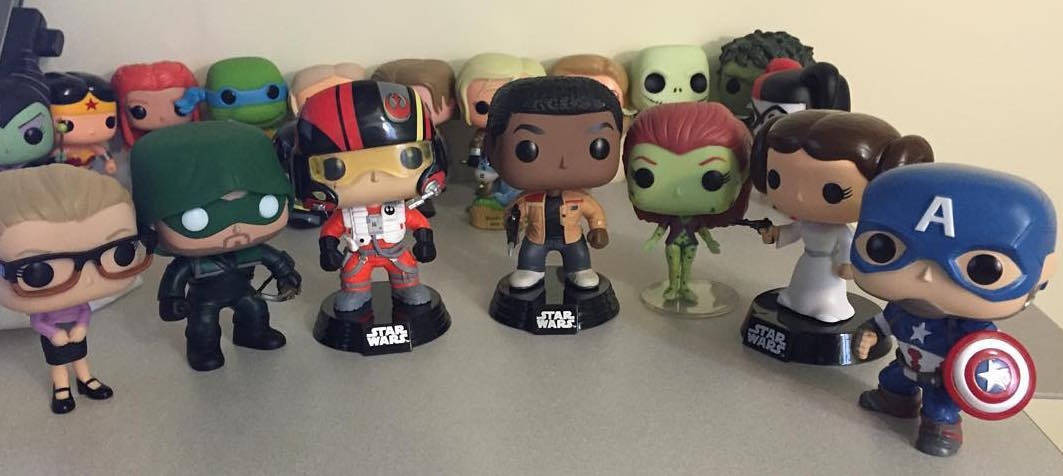
\includegraphics[width=.95\linewidth]{funko.jpg}
\caption{some Funko figs}
\end{wrapfigure}

\begin{ex}
You have 10 toy figures, but only want to place 7 of them, in an order, on the shelf. 

\vspace{5mm}

How many ways are there to order 7 of the 10 figures? 
\end{ex} 

}



\frame{ \frametitle{Permutations \#2}

\begin{defn}
The number of \textbf{permutations}\footnote{Other sources use $(n)_r$. $nPr$ is found on most calculators.} of $r$ out of $n$ distinguishable items ($r \leq n$) is 
\[ P(n,r) = nPr = \frac{n!}{(n-r)!} = n(n-1)\cdots(n-(r-1)). \]
\end{defn}

\vspace{5mm}

\textbf{Answer}: The number of ways to order 7 out of 10 figures is 
\[ P(10,7) = \frac{10!}{(10-7)!} = \frac{10!}{3!} = 10(9)(8)(7)(6)(5)(4) = 604,800. \]


}


\frame{ \frametitle{Combinations}

If order is not a concern, and all you want is the number of ways to choose $r$ out of $n$ items, then you are interested in \textbf{combinations}\footnote{Note that distinguishability is not an issue here if order does not matter.}.

\vspace{5mm}

\begin{defn}
The number of \textbf{combinations}\footnote{$nCr$ is the typical calculator notation.}\footnote{${n \choose r}$ is the typical mathematics notation.} of $r$ out of $n$ items ($r \leq n$) is 
\[ C(n,r) = nCr = {n \choose r} = \frac{n!}{r! (n-r)!}. \]
\end{defn}

\begin{notenote}
This is also said as ``$n$ choose $r$''. We'll see this value come up later as a \textbf{binomial coefficient}.
\end{notenote}

}


\frame{\frametitle{Examples: ``choose'' jumbles} 

\begin{ex}
How many jumbles are there of the word ``choose''?
\end{ex}

\vspace{5mm}

The two o's are indistinguishable, so all they need is positions. Here's a method to count: 
\begin{enumerate}
\item Choose 2 positions out of 6 to place the o's. There are ${6 \choose 2}$ ways to do this.
\item Next, there are 4 letters $\{c, e, h, s\}$ that need to be ordered in the 4 remaining spots. There are 4! ways to do this.
\end{enumerate}

}


\frame{\frametitle{Examples: ``choose'' jumbles} 

Thus, there are a total of 
\[ {6 \choose 2} \cdot 4! = \frac{6!}{2! 4!} \cdot 4! = \frac{6!}{2!} = 6(5)(4)(3) = 360 \]
ways to jumble the letters in ``choose''. 

\vspace{5mm}

Notice that the 4! canceled out - if we simply did step 2 first, the o's would have fallen immediately into place!

}


\frame{ \frametitle{Permutations vs Combinations}

To recap: the number of ways to order $r$ out of $n$ distinguishable items is the number of permutations 
\[ P(n,r) = \frac{n!}{(n-r)!} = n(n-1)\cdots(n-(r-1)). \]

\vspace{5mm} 

If order is not a concern, the number of ways to choose $r$ out of $n$ items is the number of combinations 
\[ {n \choose r} = \frac{n!}{r! (n-r)!} = \frac{P(n,r)}{r!}. \]

\vspace{5mm} 

The difference between the two is: to get rid of ``ordering'' items, divide by $r!$, since there are $r!$ ways to order $r$ items. 

}


\frame{ \frametitle{... all sorts of counting!}

You'll need to be able to combine all the following ways to correctly count spaces built from complicated experiments or situations. 

\begin{itemize}
\item multiplication principle
\item decision trees
\item Venn diagrams
\item inclusion-exclusion principle
\item permutations
\item combinations
\end{itemize}

}

\frame{ \frametitle{Pascal's triangle}

There are deep patterns underlying the binomial coefficient, or combination, function ${n \choose r}$. 

\vspace{5mm}

Many of these patterns can be seen in \textbf{Pascal's triangle} (after Blaise Pascal (1623-1662)), which displays the values of the combination function in a triangle pattern. 

}


\frame{ \frametitle{Yang Hui's / Pascal's triangle}

\begin{wrapfigure}{l}{0.3\textwidth}
\centering
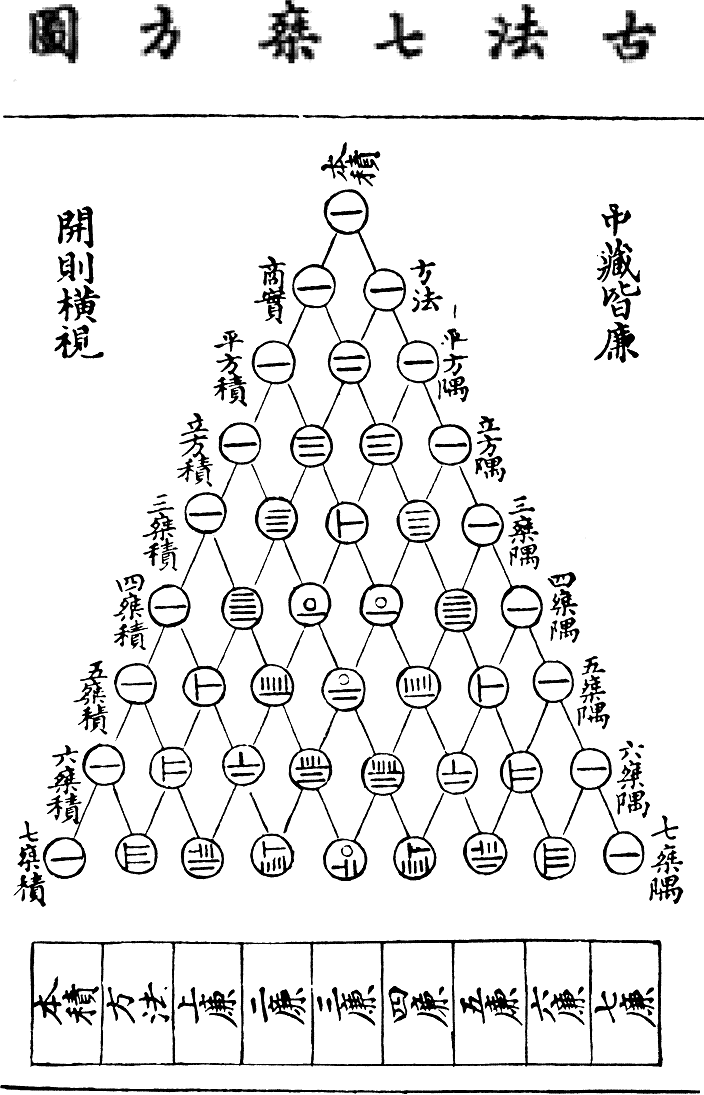
\includegraphics[width=.85\linewidth]{Yanghui_triangle.png}
\end{wrapfigure}

This triangle is named after Pascal in the Western world; however, it was known to Yang Hui, who learned it from the teachings of Jia Xian around 1100 CE, over 500 years before Pascal.

\vspace{5mm}

It was also known to Omar Khayyam (1048-1131) in Persia, and in India, in the 12th Century CE, well before it was studied by Pascal in Europe.

}


\frame{ \frametitle{Pascal's triangle}

\begin{tabular}{rcccccccccccc}
$n=0$:&    &    &    &    &    &  1\\\noalign{\smallskip\smallskip}
$n=1$:&    &    &    &    &  1 &    &  1\\\noalign{\smallskip\smallskip}
$n=2$:&    &    &    &  1 &    &  2 &    &  1\\\noalign{\smallskip\smallskip}
$n=3$:&    &    &  1 &    &  3 &    &  3 &    &  1\\\noalign{\smallskip\smallskip}
$n=4$:&    & 1 &    &  4 &    &  6 &    &  4 &    &  1\\\noalign{\smallskip\smallskip}
$n=5$:&  1 &    &  5 &    &  10 &    &  10 &    &  5 &    & 1\\\noalign{\smallskip\smallskip}
$\downarrow$ & $\downarrow$
\end{tabular}

}


\frame{ \frametitle{Pascal's triangle}

\begin{tabular}{rcccccccccccc}
$n=0$:&    &    &    &    &    &  ${0 \choose 0}$\\\noalign{\smallskip\smallskip}
$n=1$:&    &    &    &    &  ${1 \choose 0}$ &    &  ${1 \choose 1}$\\\noalign{\smallskip\smallskip}
$n=2$:&    &    &    &  ${2 \choose 0}$ &    &  ${2 \choose 1}$ &    &  ${2 \choose 2}$\\\noalign{\smallskip\smallskip}
$n=3$:&    &    &  ${3 \choose 0}$ &    &  ${3 \choose 1}$ &    &  ${3 \choose 2}$ &    &  ${3 \choose 3}$ \\\noalign{\smallskip\smallskip}
$n=4$:&    & ${4 \choose 0}$ &    &  ${4 \choose 1}$ &    &  ${4 \choose 2}$ &    &  ${4 \choose 3}$ & & ${4 \choose 4}$\\\noalign{\smallskip\smallskip}
$n=5$:&  ${5 \choose 0}$ &    &  ${5 \choose 1}$ &    &  ${5 \choose 2}$ &    &  ${5 \choose 3}$ & & ${5 \choose 4}$ & & ${5 \choose 5}$ \\\noalign{\smallskip\smallskip}
$\downarrow$ & $\downarrow$
\end{tabular}

}



\frame{ \frametitle{Combinatorial identities from Pascal's triangle}

There are several identities we can get from Pascal's triangle:\\ for $0 \leq r \leq n$, 

\begin{align*}
{n \choose r} & = {n \choose n-r} \\
\\
(\text{if } 1 \leq r \leq n) \,\, {n \choose r} & = {n-1 \choose r-1} + {n-1 \choose r} \\
\\
{n \choose m} {m \choose r} & = {n \choose r} {n-r \choose m-r} \\
\\
(\text{if } 0 \leq r < n) \,\, {n \choose r+1} & = \frac{n-r}{r+1} {n \choose r} \\
\end{align*}

}



\frame{ \frametitle{Combinatorial identities from Pascal's triangle}

There are several identities we can get from Pascal's triangle:\\ for $0 \leq r \leq n$, 

\begin{align*}
\sum_{r=0}^n {n \choose r} & = 2^n \\
\\
\sum_{r=0}^n {n \choose r}^2 & = {2n \choose n} \\
\end{align*}

}



\frame{ \frametitle{Binomial theorem}

You are familiar with \textbf{binomials}: expressions of the form $x + y$. 

\vspace{5mm}

You know how to multiply them via ``FOIL'': the square 
\[ (x+y)^2 = x^2 + 2xy + y^2. \]

In general, there are $2^n$ terms in the $n$th power of the binomial, 
\[(x+y)^n. \]

Pascal's triangle gives the coefficients in the \textbf{binomial theorem}: 

\[ (x+y)^n = \sum_{r=0}^n {n \choose r} x^r y^{n-r}. \]

}



\frame{ \frametitle{Binomial theorem}

\[ \textbf{Binomial Theorem: } (x+y)^n = \sum_{r=0}^n {n \choose r} x^r y^{n-r} \]

\vspace{5mm}

\textbf{Explanation}: Each of the $2^n$ terms is a different possible ``choice'' of ``how many $x$ get multiplied ($r$ of them)'' to ``how many $y$ ($n-r$ of them)'' to total $n$ terms in the product for that term. \\

\vspace{5mm}

How many possible ways are there to choose $r$ out of $n$ items (when order and distinguishability don't matter)? ${n \choose r}$ ways. 

}



\frame{ \frametitle{Multinomial coefficients}
Notice that, when choosing $r$ out of $n$ items, we really split the group of $n$ items into TWO groups (the $r$ you ``chose'' and the $n-r$ you ``didn't choose''). 

\vspace{5mm}

We can make this more general, splitting $n$ items into $k$ different groups, of sizes $n_1$, $n_2$, ..., $n_k$, where each $1 \leq n_i < n$ and 
\[ n_1 + n_2 + \cdots n_k = n. \]

\vspace{5mm}

This gives us the following: 

\begin{defn}
The \textbf{multinomial coefficient} gives the number of ways to divide $n$ items into $k$ groups of sizes $n_1$, $n_2$, ..., $n_k$: 
\[ { n \choose n_1, n_2, ..., n_k } = \frac{n!}{n_1! n_2! \cdots n_k!}. \]
\end{defn}

}


\frame{ \frametitle{Multinomial theorem}

Just like with the binomial theorem, multinomial coefficients are so called because they are  coefficients in the \textbf{multinomial theorem}: 

\[ (x_1 + x_2 + ... + x_k)^n = \sum_{n_1+n_2+...+n_k=n} { n \choose n_1, n_2, ..., n_k } x_1^{n_1} x_2^{n_2} \cdots x_k^{n_k}. \]

\vspace{5mm}

Note that $k=2$ gives us the old binomial coefficients and theorem: 
\[ n_1 + n_2 = n \implies {n \choose n_1, n_2} = {n \choose n_1} = {n \choose n_2} = \frac{n!}{n_1! n_2!}. \]

}



\frame{ \frametitle{Partitions}

How many ways are there to \textbf{partition} $n$ (indistinguishable) items into $k$ (distinguishable) groups?

\vspace{5mm}

In other words, how many ways are there to pick whole numbers $n_1$, $n_2$, ..., $n_k$ such that 
\[ n_1 + n_2 + ... + n_k = n? \]

\vspace{5mm}

This depends on whether or not we allow empty groups. 

}


\frame{ \frametitle{Partitions}

Both questions (empty groups or no empty groups) can be solved with an application of combinations.

\vspace{5mm}

I'll use dollar signs (\$) in the following example.

\vspace{5mm}

\begin{ex}
How many ways can we divide \$10 amongst 4 distinct people (Alice, Bob, Carol, Dave): 
\begin{itemize}
\item[(a) ] if everyone needs to get at least \$1?
\item[(b) ] if some of them can be given nothing?
\end{itemize}
\end{ex}

}



\frame{ \frametitle{Example: Partition \$10 among 4 people}

(a) \, We draw examples by counting dollars between ``bars'', which separate the different people's amounts. Listing the shares as 

\begin{center}
Alice $|$ Bob  $|$ Carol  $|$ Dave, 
\end{center}

one possible way to divide the cash is 

\[ \$\$\$\$ | \$ | \$\$\$ | \$\$ \]

\begin{center}
Alice gets \$4  $|$ Bob gets \$1  $|$ Carol gets \$3 $|$ Dave gets \$2. 
\end{center}

This is different from 

\[ \$\$\$\$ | \$\$ | \$\$\$ | \$ \]

\begin{center}
Alice gets \$4  $|$ Bob gets \$2  $|$ Carol gets \$3 $|$ Dave gets \$1. 
\end{center}

}


\frame{ \frametitle{Partitions \#1: Everybody gets at least one}

How many ways are there to make these sequences of \$ and $|$, so that each person gets at least \$1?

\vspace{5mm}

We have 10 \$ symbols to place in sequence, and 4-1 = 3 bars $|$ to place \emph{between} \$ to make sure that at least one \$ is in each set. Hence, there are 10-1 = 9 positions to place the bars in. (Why?)

\vspace{5mm}

Thus, the number of partitions of \$10 into 4 nonempty sets is 
\[ {10-1 \choose 4-1} = {9 \choose 3} = \frac{9!}{3! 6!} = \frac{9(8)(7)}{3(2)(1)} = 84. \]

}



\frame{ \frametitle{Partitions \#1: Everybody gets at least one}

The number of partitions of $n$ items into $k$ labeled nonempty sets is 
\[ {n-1 \choose k-1}. \]


}


\frame{ \frametitle{Partitions \#2: Maybe not everybody gets at least one?}

(b) \, What if we don't care if someone goes without? 

\vspace{5mm}

There should be a lot more ways to partition the money if some people might get nothing.

\vspace{5mm}

In this case, we have no restrictions on where to place the bars in the sequence of symbols - they are not restricted to being between dollar signs. 

} 


\frame{ \frametitle{Partitions \#2: Maybe not everybody gets at least one?}

For example, we could just give all the money to Alice: 

\[ \$\$\$\$\$\$\$\$\$\$||| \]

In this case, we have \$10 and 4-1 = 3 bars, for a total of 
\[ 10+3 = 13 \] 
symbols in a sequence, and all we need to do is place the 3 bars and the dollars will fall into place.

\vspace{5mm}

The number of 3-combinations out of 13 items is 
\[ {10+3 \choose 3} = {13 \choose 3} = \frac{13!}{3! 10!} = \frac{13(12)(11)}{3(2)(1)} = 286. \]




}

\frame{ \frametitle{Partitions \#2: Maybe not everybody gets at least one?}

The number of partitions of $n$ items into $k$ labeled sets \emph{with possible empty sets} is 
\[ {n+k-1 \choose k-1}. \]

\vspace{5mm}

This is larger than with the restriction that every set be nonempty: 

\[ {n+k-1 \choose k-1} \geq {n-1 \choose k-1}. \]

}



\frame{ \frametitle{``Derangements''}

An ordering of $n$ items is called an ``arrangement''. 

\vspace{5mm}

Sometimes there is a ``right order'' for a list of $n$ items. 

\vspace{5mm}

However, if a list of $n$ items is in such an order that \emph{none of the items is in the ``right'' place}, we call the list a ``derangement''. 

\vspace{5mm}

How many ways are there to have a ``derangement'' of $n$ items?


}


\frame{ \frametitle{Derangements: The wrong envelopes problem}

After a birthday party, you write 10 personalized thank you cards for gifts you've received.

\vspace{5mm}

Somehow, the cards and their pre-addressed envelopes get mixed up, and, not paying attention, you place the cards in randomly- addressed envelopes. 

\vspace{5mm}

How many ways is it possible that NONE of the 10 people you mail to gets the card you wrote them? 

}


\frame{ \frametitle{Derangements: The wrong envelopes problem}

To solve this, we'll go back to the inclusion-exclusion principle. 

\vspace{5mm}

\[ \left| \bigcup_{i=1}^n A_i \right| = \sum_{i=1}^n |A_i| - \sum_{i \neq j, i,j=1}^n |A_i \cap A_j| + \cdots + (-1)^{n+1}  \left| \bigcap_{i=1}^{n} A_i \right| \]

 }
 
   
\frame{ \frametitle{Derangements: The wrong envelopes problem}

Let $A_i$ be the set of arrangements where card $i$ is wrongly placed.

\vspace{5mm}

We want to know the cardinality 
\[ \left| \bigcap_{i=1}^{n} A_i \right| \]
where all $n$ cards are misplaced.

}


\frame{ \frametitle{Derangements: The wrong envelopes problem}

Knowing that there are a total of $n!$ arrangements of $n$ cards, and using inclusion-exclusion, we have 

\begin{align*} 
\left| \bigcap_{i=1}^{n} A_i \right| = & n! - (-1)^{n+1}\bigg(\left| \bigcup_{i=1}^n A_i \right| - \sum_{i=1}^n |A_i| + \sum_{i \neq j, i,j=1}^n |A_i \cap A_j| \\
 & - \cdots - (-1)^{n} \sum_{n-1 \text{ wrong}} |\cap A_i|\bigg).
\end{align*}

While this looks messy, we can go term by term.

}


\frame{ \frametitle{Derangements: The wrong envelopes problem}

First, $\left| \bigcup_{i=1}^n A_i \right|$ is the number of ways that at least one is wrong.

\vspace{5mm}

Since there is \emph{only one way} to get all of them right, 
\[ \left| \bigcup_{i=1}^n A_i \right| = n! - 1. \]

\vspace{5mm}

Next, $|A_i|$ is the number of ways to get card $i$ wrong (ignoring the others). This is simply 
\[ |A_i| = (n-1) \cdot (n-1)! \]
since you pick one of the $n-1$ incorrect envelopes for card $i$, and then any of the $(n-1)!$ orderings for the others. 

}


\frame{ \frametitle{Derangements: The wrong envelopes problem}

Carefully proceeding in this way, we can find that the number of derangements of $n$ items, denoted 

\[ !n \] 

(as an homage to the factorial notation of arrangements), 

\[ !n := n! \sum_{i=0}^n \frac{(-1)^i}{i!}. \]

}


\frame{ \frametitle{Derangements}

A few calculations are given below. 

\vspace{5mm}

\begin{align*}
!2 & = 2! \left(1-1+\frac{1}{2} \right) & = & 1 \\
!3 & = 3! \left(1-1+\frac{1}{2} - \frac{1}{6}\right) & = & 2 \\
!4 & = 4! \left(1-1+\frac{1}{2} - \frac{1}{6} + \frac{1}{24}\right) & = & 9 \\
!10 & = 10! \sum_{i=0}^{10} \frac{(-1)^i}{i!} & = & 1,334,961.
\end{align*}
% https://oeis.org/A000166
}


\end{document}
